%%%%%%%%%%%%%%%%%%%%%%%%%%%%%%%%%%%%%%%%%%%%%%%%%%%%%%%%%%%%%%
%% LaTeX template for the science justification to be       %%
%%     submitted as part of a regular ALMA proposal.        %%
%% This template should also be used for a ToO, DDT, or     %%
%%     mm-VLBI ALMA proposal, but NOT for Large Programs    %%
%%     (these have a separate template with more sections)  %%
%%                                                          %%
%%                      ALMA Cycle 8 2021                   %%
%%                                                          %%
%%%%%%%%%%%%%%%%%%%%%%%%%%%%%%%%%%%%%%%%%%%%%%%%%%%%%%%%%%%%%%

%%%%%%%%%%%%%%%%%%%%%%%%%%%%%%%%%%%%%%%%%%%%%%%%%%
%%%%% How to convert this document to PDF %%%%%%%%
%%%%%%%%%%%%%%%%%%%%%%%%%%%%%%%%%%%%%%%%%%%%%%%%%%

% If your figures are stored as PostScript files, you can use the 
% following commands to generate a PDF file of your proposal:

%% latex file.tex
%% dvips file.dvi
%% ps2pdf file.ps file.pdf 


% If your figures are PDF images or bitmap pictures in PNG, JPG, or GIF format,
% you can use the pdflatex command to generate a PDF file from this template
% (note, however, that the pdflatex command does not handle PostScript files):

% pdflatex file.tex

% Warnings: 
%           1. You must make sure that PDF output generated from this
%              template is complete both when displayed with a viewer 
%              (acroread, for example) and when printed on paper.
%              LaTeX installations vary greatly and therefore it might 
%              not be possible to get all proposals to come out 
%              correctly with a single text page layout. 
%              In some cases you will have to adjust the 
%              \topmargin=-7mm command in the template to center the 
%              text vertically in the page.  
%           2. The scientific justification, figures, tables, references,
%              and public outreach statement must all fit within the
%              4-page limit.
%           3. You are free to include colour images in your proposal justification.
%              Proposals are distributed to ALMA Review Panels and to distributed
%              peer review reviewers in electronic form.
%              However, the scientific content of the images should still remain
%              clear when displayed or printed in black and white.
%           4. This template is for regular, ToO, DDT, or mm-VLBI ALMA proposals,
%              but NOT for Large Programs: these have a separate template with
%              more sections, and is available from the ALMA Science Portal


%%%%%%%%%%%%%%%%%%%%%%%%%%%%%%%%%%%%%%%%%%%%%%
%%%%% Default format: 12pt single column %%%%%
%% 12pt is the minimum font size allowed !! %%
%% This applies to everything, including    %%
%% references, figure captions, and tables  %%
%% ==> Proposals not compliant to this will %%
%%     be rejected. See Section 5.3.1 in    %%
%%     the ALMA Proposer's Guide            %%
%%%%%%%%%%%%%%%%%%%%%%%%%%%%%%%%%%%%%%%%%%%%%%

\documentclass[12pt,a4paper]{article}  %% DO NOT CHANGE to 11pt or less !

\usepackage[dvipdfmx]{graphics, graphicx}
% if you on overleaf...
\usepackage{color}
% if you on local...
% \usepackage[dvipdfmx]{color}
\usepackage{amsmath,amssymb}
\usepackage{natbib}
\usepackage{aas_macros}
\usepackage{compactbib}
\usepackage{txfonts}
\usepackage{threeparttable}

%%%%%%%%%%%%%%%%%%%%%%%%%%%%
%%%%%% Page dimensions %%%%%
%%%%%%  DO NOT CHANGE  %%%%%
%%%%%%%%%%%%%%%%%%%%%%%%%%%%

\textheight=247mm
\textwidth=180mm
\topmargin=-7mm
\oddsidemargin=-10mm
\evensidemargin=-10mm
\parindent 10pt

%%%%%%%%%%%%%%%%%%%%%%%%%%%%%
%%%%% Start of document %%%%% 
%%%%%%%%%%%%%%%%%%%%%%%%%%%%%

\begin{document}
\pagestyle{plain}
\pagenumbering{arabic}
 
% The title, abstract and list of investigators should NOT be included in the
% Scientific justification. The title and abstract are put automatically on the cover page.

%%%%%%%%%%%%%%%%%%%%%%%%%%%%%%%%%%%%%%%%%
%%%%% Body of science justification %%%%%
%%%%%%%%%%%%%%%%%%%%%%%%%%%%%%%%%%%%%%%%%

%% ENTER TEXT, FIGURES AND TABLES BELOW
%% Minimum font size for all text, references, figure captions, and tables is 12pt
%% Proposals not compliant to this will be rejected. See Section 5.3.1 in the ALMA Proposer's Guide.

\section{Scientific Justification}
Nogizaka 46 is the most popular idol group in Japan \citep{Yamato22}.

\begin{figure*}[h]
    \centering
    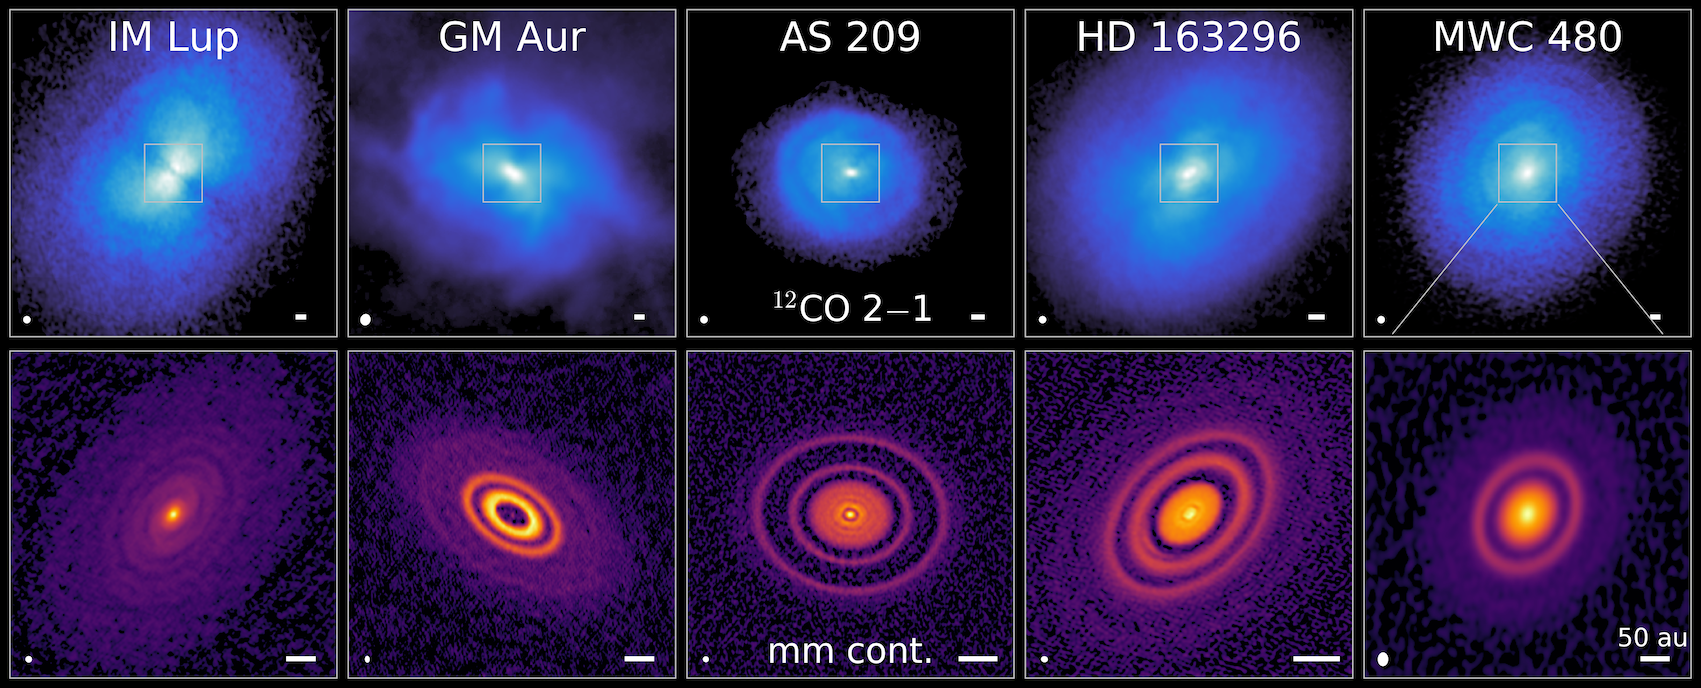
\includegraphics[width=0.8\hsize]{MAPS_disks.png}
    \caption{\em{Hogehoge}}
    \label{fig:MAPS_disks}
\end{figure*}

\section{Description of Observations}
Shiori Kubo is a very attractive member of Nogizaka 46 \citep{Yamato23}.

% Please describe the observations to be made and their specific
% purpose, with a clear explanation of the need for, and 
% appropriateness of, ALMA Cycle 8 2021 data.  


%\section{References}
% List references here
% Minimum font size for references: 12pt 
% Proposals not compliant to this will be rejected. See Section 5.3.1 in the ALMA Proposer's Guide.

\section*{References}
\bibliographystyle{aas_compactbib}
\bibliography{reference}

\end{document}